% Template created by Karol Kozioł (www.karol-koziol.net) for ShareLaTeX

\documentclass[a4paper,9pt]{extarticle}
\usepackage[utf8]{inputenc}
\usepackage[T1]{fontenc}
\usepackage{graphicx}
\usepackage{xcolor}
\usepackage{tikz}
\usepackage{enumitem}
\setlist{nosep}

\usepackage{amsmath,amssymb,textcomp}
\everymath{\displaystyle}

\usepackage{times}
\renewcommand\familydefault{\sfdefault}
\usepackage{tgheros}
\usepackage[defaultmono,scale=0.85]{droidmono}

\usepackage{multicol}
\setlength{\columnseprule}{0pt}
\setlength{\columnsep}{20.0pt}


\usepackage{geometry}
\geometry{a4paper,left=10mm,right=10mm,top=10mm,bottom=15mm}

\linespread{1.3}


% custom title
\makeatletter
\renewcommand*{\maketitle}{%
\noindent
\begin{minipage}{0.4\textwidth}

\begin{tikzpicture}
\node[rectangle,rounded corners=6pt,inner sep=10pt,fill=blue!50!black,text width= 0.95\textwidth] {\color{white}\Huge \@title};
\end{tikzpicture}
\end{minipage}
\hfill
\begin{minipage}{0.55\textwidth}
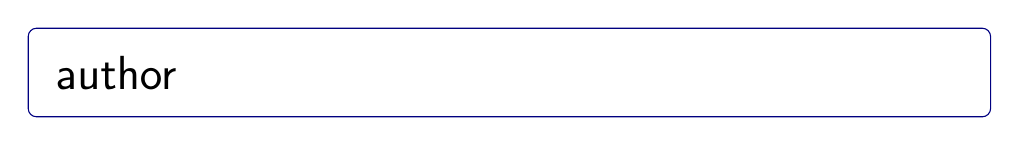
\begin{tikzpicture}
\node[rectangle,rounded corners=3pt,inner sep=10pt,draw=blue!50!black,text width= 0.95\textwidth] {\LARGE \@author};
\end{tikzpicture}
\end{minipage}
\bigskip\bigskip
}%
\makeatother

% custom section
\usepackage[explicit]{titlesec}
\newcommand*\sectionlabel{}
\titleformat{\section}
  {\gdef\sectionlabel{}
   \normalfont\sffamily\Large\bfseries\scshape}
  {\gdef\sectionlabel{\thesection\ }}{0pt}
  {
\noindent
\begin{tikzpicture}
\node[rectangle,rounded corners=3pt,inner sep=4pt,fill=blue!50!black,text width= 0.95\columnwidth] {\color{white}\sectionlabel#1};
\end{tikzpicture}
  }
\titlespacing*{\section}{0pt}{15pt}{10pt}


% custom footer
\usepackage{fancyhdr}
\makeatletter
\pagestyle{fancy}
\fancyhead{}
\fancyfoot[C]{\footnotesize \textcopyright\ \@date\ \ \@author}
\renewcommand{\headrulewidth}{0pt}
\renewcommand{\footrulewidth}{0pt}
\makeatother


\title{Biol 461 Section 01/08/21}
\author{Nernst Equation and the Resting Membrane Potential}
\date{01/09/2021}



\begin{document}

\maketitle

\begin{multicols*}{2}


\section*{Nernst Equation}

\[E_{ion} = \frac{RT}{FZ}*\ln(\frac{[ion]_{out}}{[ion]_{in}})\]

\begin{itemize}
\setlength\itemsep{.5em}
  \item $E_{ion}$ is the equilibrium (or reversal) potential of the ion
  \item $R$ is the gas constant (energy per temperature increment per mole)
  \item $T$ is the temperature in Kelvin
  \item $F$ is the Faraday constant (magnitude of electrical charge per mole of electrons)
  \item $Z$ is the valence (charge) of the ion
  \item $[ion_{in}]$ and $[ion_{out}]$ are the intracellular and extracellular ion concentrations respectively
\end{itemize}


\section*{What does the Nernst Equation Tell Us?}

The membrane potential at which the diffusional force and electrical force on an ion are equal. At this membrane potential, if the membrane is permeable to the ion in question, the rate of ions leaving the cell is equal to the rate of ions entering the cell.
%Ions are affected by concentration gradients and electrical gradients. 
%The force on an ion caused by its concentration gradient is %$RT*\ln(\frac{[ion]_{out}}{[ion]_{in}})$ \\
%The force on an ion from the electrical gradient is $V_m*FZ$ where $V_m$ is the overall membrane voltage. When calculatino 

%The equilibrium potential is the membrane potential at which the diffusional and electrical forces on an ion are equal. 

\section*{Goldman-Hodgkin-Katz Equation}

$V_{mem} = \frac{RT}{F}*\ln(\frac{P_{K} * [K^+]_{out} + P_{Na} * [Na^+]_{out} + P_{Cl} * [Cl^-]_{out}}{P_{K}*[K^+]_{in} + P_{Na} * [Na^+]_{in} + P_{Cl} * [Cl^-]_{in}})$
\\
\begin{itemize}
\setlength\itemsep{.5em}
  \item $V_{mem}$ is the membrane potential
  \item $P_{ion x}$ is the relative permeability of the membrane to ion x.
  \item NOTE: This is only the equation for monovalent ions.
\end{itemize}


\section*{What does the Goldman-Hodgkin-Katz \\Equation tell us?}

Given the reversal potentials of all monovalent ions that can pass through a cell membrane and the membrane's relative permeability to each of the ions, the Goldman-Hodgkin-Katz Equation tells us the overall voltage difference across the cell membrane (Vmem).

\vfill\null
\columnbreak 
\section*{Practice Questions}
\begin{enumerate}
  \item A model cell has an intracellular chloride concentration of 5mM and an extracellular chloride concentration of 120mM. At room temperature what is the reversal potential for chloride?
  \item \begin{enumerate}
     \item A model cell has an intracellular potassium concentration of 125mM and an extracellular potassium concentration of 4mM. At room temperature what is the reversal potential for potassium?
     \item This same model cell has an extracellular sodium concentration of 140mM and an intracellular sodium concentration of 10 mM. What is the reversal potential for sodium?
     \item Assume the membrane is only permeable to sodium and potassium. 95\% of the membrane's resting permeability is specific for potassium and 5\% of the membrane's resting permeability is specific for sodium. What is the resting membrane potential of the cell?
     \item I increase the extracellular concentration of potassium to 70mM. What is the new reversal potential for potassium? 
     \item What is the new membrane potential of the cell? Is this hyperpolarized or depolarized in comparison to the previously calculated membrane potential?
     \item Assume I put the cell back in the 4mM potassium extracellular solution (so that the membrane potential is what you calculated in part c) and now I open a bunch of sodium channels such that the membrane becomes 70\% permeable to sodium and 30\% permeable to potassium. What is the membrane potential of the cell under these new conditions? Is this hyperpolarized or depolarized in comparison to the membrane potential you calculated in part C?
     \end{enumerate}
\end{enumerate}

\end{multicols*}

\end{document}
